\documentclass[hidelinks,english]{article}

\usepackage{graphicx}
\usepackage{grffile}
\usepackage[T1]{fontenc}
\usepackage{babel}
\usepackage{wrapfig}
\usepackage{hyperref}
\usepackage{amsmath}

\date{\today}

\graphicspath{{Pictures/}}
\begin{document}	
	\begin{titlepage}
		\pagenumbering{gobble}
		\begin{figure}[!t]
			
\includegraphics[width=\linewidth]{up_logo.png}
		\end{figure}
		\vspace*{\stretch{1.0}}
		\begin{center}
			\huge{COS 314: Artificial Intelligence}\\
			\large{Project 2: Neural Networks}\\
			\vspace{10mm}
		\end{center}
		\begin{center}
			\huge\begin{tabular}{ c }
				Maree, Armand\\
				\texttt{120 178 00}
			\end{tabular}
		\end{center}
		\begin{center}
			Department of Computer Science, University of Pretoria\\
			\today
		\end{center}
		\vspace*{\stretch{2.0}}
	\end{titlepage}
	\newpage
	\tableofcontents
	\newpage
	\pagenumbering{arabic}
	
	\section{Code and Compilation}\label{compilation}
		\paragraph\indent
		The Neural Network (NN) was coded in Java\footnote{Oracle Java was used to test the program and no guarantee can be made for any Java distributions.} and is located in the subdirectory called "NeuralNetwork". Each of the experiments is located in this directory as "Experiment1", "Experiment2" and "Experiment3". In order to compile and run a project simply run the command "make all" in the terminal of a Linux machine. This will compile, run and clean the directory.
		
	\section{Stopping Conditions}
		\paragraph\indent
		The NN is stopped as soon as the generalisation accuracy reaches 99\% or when the NN starts over fitting. An epoch maximum was specified at 1000 for experiment 1 and 2. This was to allow the NN to to reach the best possible values it can, but if one has to wait ages for the result then it is useless. Experiment 3, however, was allowed to run until 3000 epochs to allow it more time since it is more complex.
		
	\section{Experiment 1}
		\subsection{Usage}
			\paragraph\indent
			Once the NN has started executing (see section \ref{compilation}) the user will be prompted (in the terminal) to type a specific letter. This will be the letter that the NN attempts to learn the pattern for. Statistics will be printed to the screen after each epoch\footnote{Processing the training set once.}. Similar statistics will be written to the a file called "NNStats.txt".
			
		\subsection{Results}
			\paragraph\indent
			Table \ref{table:exp1results} shows the average results over 30 sessions for each of the 16 test cases that was run on the NN for the letter 'A'. The columns are described as follows: \(\epsilon\) (epoch of solution), HU\footnote{Number of neurons in the single hidden layer.} (number of hidden units), \(\eta\) (learning rate) , \(\alpha\) (momentum), TE\footnote{Percentage incorrect classifications in the training set.} (training error), GE (generalisation error).
			\begin{table}[!h]
				\centering
				\begin{tabular}{||c | c | c | c | c | c||} 
					\hline
					\(\epsilon\) & HU & \(\eta\) & \(\alpha\) & TE (\%) & GE (\%) \\ [0.5ex] 
					\hline\hline
					7.2 & 5 & 0.1 & 0.1 & 1.1 & 0.9 \\ 
					\hline
					3.5 & 5 & 0.2 & 0.2 & 1.1 & 0.9 \\ 
					\hline
					2.3 & 5 & 0.3 & 0.3 & 1.1 & 0.8 \\ 
					\hline
					1.8 & 5 & 0.4 & 0.4 & 1.1 & 1.0 \\ 
					\hline
					6.5 & 10 & 0.1 & 0.1 & 1.1 & 0.9 \\ 
					\hline
					3.1 & 10 & 0.2 & 0.2 & 1.1 & 0.9 \\ 
					\hline
					2.1 & 10 & 0.3 & 0.3 & 1.1 & 0.8 \\ 
					\hline
					1.5 & 10 & 0.4 & 0.4 & 1.1 & 0.9 \\ 
					\hline
					6.8 & 15 & 0.1 & 0.1 & 1.1 & 0.9 \\ 
					\hline
					3.3 & 15 & 0.2 & 0.2 & 1.1 & 0.9 \\ 
					\hline
					1.9 & 15 & 0.3 & 0.3 & 1.1 & 0.8 \\ 
					\hline
					1.3 & 15 & 0.4 & 0.4 & 1.2 & 0.9 \\ 
					\hline
					6.6 & 20 & 0.1 & 0.1 & 1.1 & 0.9 \\ 
					\hline
					3.2 & 20 & 0.2 & 0.2 & 1.1 & 0.9 \\ 
					\hline
					2.1 & 20 & 0.3 & 0.3 & 1.1 & 0.9 \\ 
					\hline
					1.5 & 20 & 0.4 & 0.4 & 1.1 & 0.9 \\ 
					\hline
				\end{tabular}
				\caption{Experiment 1 test results}
				\label{table:exp1results}
			\end{table}
			\paragraph\indent
			As seen from table \ref{table:exp1results}, 15 hidden units (HU), a learning rate (\(\eta\)) of 0.3 and a momentum (\(\alpha\)) of 0.3 are the optimal values for this NN. This gives the fastest result and also the best accuracy.
			\paragraph\indent
			In figure \ref{fig:exp1graph} the change in the accuracy can be seen as the epochs increase.
			\begin{figure}[!t]
				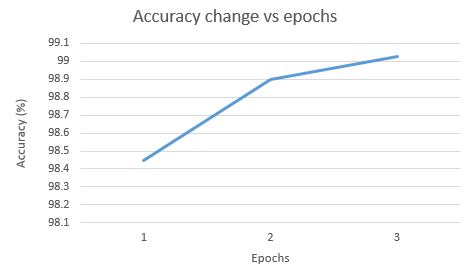
\includegraphics[width=\linewidth]{experiment1.png}
				\caption{Experiment 1 accuracy over epoch.}
				\label{fig:exp1graph}
			\end{figure}
			
	\section{Experiment 2}
		\subsection{Usage}
			\paragraph\indent
			Once the program has started executing (see section \ref{compilation}) the NN will immediately start learning to identify the all vowels. Statistics will be printed to the screen after each epoch. Similar statistics will be written to the a file called "NNStats.txt".
			
		\subsection{Results}
			\paragraph\indent
			Table \ref{table:exp2results} shows the average results over 30 sessions for each of the 16 test cases that was run on the NN for all vowels. The columns are described as follows: \(\epsilon\) (epoch of solution), HU (number of hidden units), \(\eta\) (learning rate) , \(\alpha\) (momentum), TE (training error), GE (generalisation error).
			\begin{table}[!h]
				\centering
				\begin{tabular}{||c | c | c | c | c | c||} 
					\hline
					\(\epsilon\) & HU & \(\eta\) & \(\alpha\) & TE (\%) & GE (\%) \\ [0.5ex] 
					\hline\hline
					85.2 & 5 & 0.1 & 0.1 & 22.3 & 25.0 \\ 
					\hline
					59.6 & 5 & 0.2 & 0.2 & 14.2 & 16.7 \\ 
					\hline
					41.0 & 5 & 0.3 & 0.3 & 13.9 & 16.5 \\ 
					\hline
					19.5 & 5 & 0.4 & 0.4 & 15.4 & 18.8 \\ 
					\hline
					258.0 & 10 & 0.1 & 0.1 & 11.2 & 13.2 \\ 
					\hline
					138.2 & 10 & 0.2 & 0.2 & 8.7 & 10.2 \\ 
					\hline
					73.9 & 10 & 0.3 & 0.3 & 9.3 & 11.5 \\ 
					\hline
					44.2 & 10 & 0.4 & 0.4 & 10.4 & 13.8 \\ 
					\hline
					454.1 & 15 & 0.1 & 0.1 & 6.1 & 7.2 \\ 
					\hline
					187.8 & 15 & 0.2 & 0.2 & 6.5 & 8.0 \\ 
					\hline
					76.9 & 15 & 0.3 & 0.3 & 8.1 & 10.9 \\ 
					\hline
					42.6 & 15 & 0.4 & 0.4 & 10.0 & 13.9 \\ 
					\hline
					440.0 & 20 & 0.1 & 0.1 & 5.1 & 7.0 \\ 
					\hline
					252.5 & 20 & 0.2 & 0.2 & 5.2 & 7.4 \\ 
					\hline
					102.6 & 20 & 0.3 & 0.3 & 7.0 & 10.1 \\ 
					\hline
					42.7 & 20 & 0.4 & 0.4 & 9.2 & 13.3 \\ 
					\hline
				\end{tabular}
				\caption{Experiment 2 test results}
				\label{table:exp2results}
			\end{table}
			\paragraph\indent
			As seen from the table \ref{table:exp2results}, 20 hidden units (HU), a learning rate (\(\eta\)) of 0.2 and a momentum (\(\alpha\)) of 0.2 are the optimal values for this NN. It provides the second best results (the difference between first place and second place is nearly neglectable) in a reasonable amount of time.
			\paragraph\indent
			In figure \ref{fig:exp2graph} the change of the incorrect classifications can be seen as the epochs increase.
			\begin{figure}[!t]
				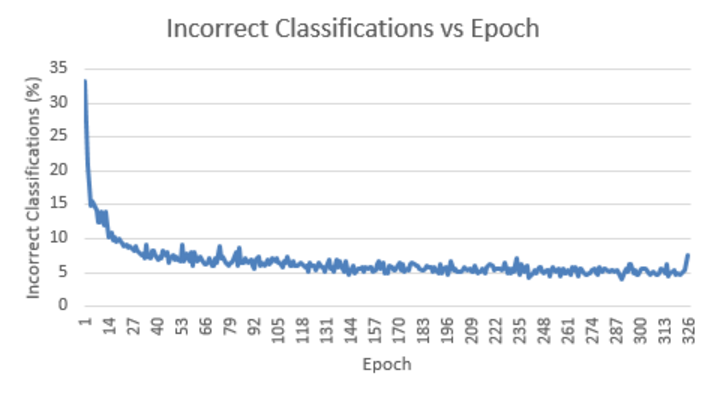
\includegraphics[width=\linewidth]{experiment2.png}
				\caption{Experiment 2 incorrect classifications over epoch.}
				\label{fig:exp2graph}
			\end{figure}	
	
	\section{Experiment 3}
		\subsection{Usage}
			\paragraph\indent
			Once the program has started executing (see section \ref{compilation}) the NN will immediately start learning to identify the all alphabet characters. Statistics will be printed to the screen after each epoch. Similar statistics will be written to the a file called "NNStats.txt".
			
		\subsection{Results}
			\paragraph\indent
			Table \ref{table:exp3results} shows the average results over 30 sessions for each of the 16 test cases that was run on the NN for all vowels. The columns are described as follows: \(\epsilon\) (epoch of solution), HU (number of hidden units), \(\eta\) (learning rate) , \(\alpha\) (momentum), TE (training error), GE (generalisation error).
			\begin{table}[!h]
				\centering
				\begin{tabular}{||c | c | c | c | c | c||} 
					\hline
					\(\epsilon\) & HU & \(\eta\) & \(\alpha\) & TE (\%) & GE (\%) \\ [0.5ex] 
					\hline\hline
					538.2 & 5 & 0.1 & 0.1 & 66.3 & 66.7 \\ 
					\hline
					204.4 & 5 & 0.2 & 0.2 & 68.1 & 69.4 \\ 
					\hline
					108.3 & 5 & 0.3 & 0.3 & 67.5 & 69.3 \\ 
					\hline
					66.8 & 5 & 0.4 & 0.4 & 68.5 & 70.0 \\ 
					\hline
					460.9 & 10 & 0.1 & 0.1 & 41.0 & 41.5 \\ 
					\hline
					213.8 & 10 & 0.2 & 0.2 & 41.0 & 42.3 \\ 
					\hline
					110.7 & 10 & 0.3 & 0.3 & 41.5 & 43.1 \\ 
					\hline
					71.0 & 10 & 0.4 & 0.4 & 42.4 & 44.3 \\ 
					\hline
					689.9 & 15 & 0.1 & 0.1 & 31.9 & 32.4 \\ 
					\hline
					240.9 & 15 & 0.2 & 0.2 & 33.4 & 34.8 \\ 
					\hline
					150.0 & 15 & 0.3 & 0.3 & 33.5 & 34.8 \\ 
					\hline
					79.2 & 15 & 0.4 & 0.4 & 35.0 & 37.0 \\ 
					\hline
					661.2 & 20 & 0.1 & 0.1 & 27.9 & 28.3 \\ 
					\hline
					303.9 & 20 & 0.2 & 0.2 & 28.8 & 29.3 \\ 
					\hline
					180.2 & 20 & 0.3 & 0.3 & 28.9 & 30.3 \\ 
					\hline
					103.9 & 20 & 0.4 & 0.4 & 29.8 & 31.3 \\ 
					\hline
				\end{tabular}
				\caption{Experiment 3 test results}
				\label{table:exp3results}
			\end{table}
			
			\paragraph\indent
			Due to the bad nature of these results I have decided to run another few tests to see if a better result could be obtained. These results are listed in table \ref{table:exp3results2}.
			
			\begin{table}[!h]
				\centering
				\begin{tabular}{||c | c | c | c | c | c||} 
					\hline
					\(\epsilon\) & HU & \(\eta\) & \(\alpha\) & TE (\%) & GE (\%) \\ [0.5ex] 
					\hline\hline
					1384.9 & 35 & 0.1 & 0.1 & 18.3 & 19.0 \\ 
					\hline
					548.2 & 35 & 0.2 & 0.2 & 19.8 & 20.6 \\ 
					\hline
					312 & 35 & 0.3 & 0.3 & 21.2 & 22.3 \\ 
					\hline
					189.1 & 35 & 0.4 & 0.4 & 22.4 & 23.9 \\ 
					\hline
					2598 & 40 & 0.1 & 0.1 & 15.1 & 15.5 \\ 
					\hline
					594.3 & 40 & 0.2 & 0.2 & 18.3 & 18.8 \\ 
					\hline
					431 & 40 & 0.3 & 0.3 & 19.0 & 19.5 \\ 
					\hline
					318.3 & 40 & 0.4 & 0.4 & 20.2 & 21.2 \\ 
					\hline
				\end{tabular}
				\caption{Experiment 3 test results}
				\label{table:exp3results2}
			\end{table}
			
			\paragraph\indent
			As seen from the table \ref{table:exp3results2}, 40 hidden units (HU), a learning rate (\(\eta\)) of 0.1 and a momentum (\(\alpha\)) of 0.1 are the optimal values for this NN if accuracy is the priority. If speed is the priority, a learning rate and momentum of 0.3 should be applied to 40 hidden units.
			
			\paragraph\indent
			In figure \ref{fig:exp3graph} the change of the incorrect classifications can be seen as the epochs increase for the latter case in the previous paragraph.
			\begin{figure}[!t]
				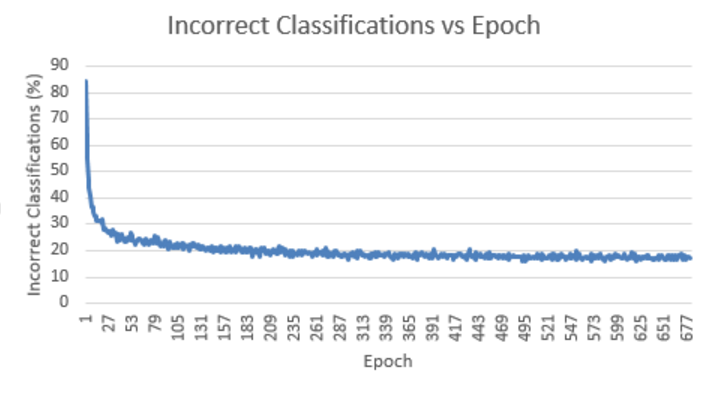
\includegraphics[width=\linewidth]{experiment3.png}
				\caption{Experiment 3 incorrect classifications over epoch.}
				\label{fig:exp3graph}
			\end{figure}
			
\end{document}
